\documentclass[lettersize,journal]{IEEEtran}
\usepackage{amsmath,amsfonts}
\usepackage{algorithm}
\usepackage{algpseudocode}
\usepackage{array}
\usepackage[caption=false,font=normalsize,labelfont=sf,textfont=sf]{subfig}
\usepackage{textcomp}
\usepackage{stfloats}
\usepackage{url}
\usepackage{graphicx}
\usepackage{float}
\usepackage{cite}
\usepackage{balance}
\usepackage[colorlinks=true,linkcolor=blue]{hyperref}
\usepackage{listings}
\usepackage{booktabs} % 用于专业排版的表格宏包
\usepackage{multirow} % 用于合并单元格的宏包
\hyphenation{op-tical net-works semi-conduc-tor IEEE-Xplore}
\def\BibTeX{{\rm B\kern-.05em{\sc i\kern-.025em b}\kern-.08em
    T\kern-.1667em\lower.7ex\hbox{E}\kern-.125emX}}

\begin{document}

\title{Video Retrieval of Autonomous Driving Scenarios Based on Large Models}
\author{12310520 Rui Yuhan   12310437 Qiao Shihan}


\maketitle

\begin{abstract}
Video retrieval in autonomous driving scenarios demands models to comprehend complex visual environments and align them with detailed textual descriptions. While multimodal large language models (MLLMs) have demonstrated potential in vision-language tasks, their application to domain-specific video retrieval remains underexplored. Furthermore, the scarcity of publicly available high-quality annotated video data in the autonomous driving domain makes it challenging for models to accurately learn video content semantics from limited data. Additionally, significant differences exist between autonomous driving videos and those in general video datasets, leading to suboptimal performance of generic large models on autonomous driving datasets.

To address these challenges, we evaluate the performance of two distinct pretrained MLLMs on a carefully curated autonomous driving dataset. This dataset features high-quality captions that have undergone multi-round optimization, combining human annotation expertise with advanced automated labeling techniques, while also serving as a benchmark platform for exploring more efficient annotation strategies. Experimental results demonstrate that our approach effectively retrieves relevant video segments based on textual queries, highlighting the potential of MLLMs to enhance retrieval accuracy and scalability.

\end{abstract}

\begin{IEEEkeywords}
Autonomous Driving Video Retrieval, Multimodal Large Language Models (MLLMs), Video Understanding, Automated Annotation Optimization
\end{IEEEkeywords}

\begin{figure*}
    \centering
    \includegraphics[width=1\linewidth]{images/structure.jpg}
    \caption{The structure of our work}
    \label{fig:1}
\end{figure*}

\section{Introduction}

Autonomous driving systems require advanced models capable of comprehending complex visual scenes and retrieving relevant video segments based on textual queries. Although multimodal large language models (MLLMs) have demonstrated outstanding performance in general vision-language tasks, their application in domain-specific video retrieval for autonomous driving remains underexplored. This research gap is further exacerbated by the lack of high-quality annotated datasets that integrate visual, textual, and action information - all of which are crucial for training robust models. Existing datasets often lack detailed annotations or fail to capture the complex reasoning processes required in autonomous driving scenarios, limiting the models' generalization capability in real-world applications.

To address these challenges, we propose an attempt at automated dataset annotation and conduct experiments on our self-constructed dataset, leveraging the advantages of pretrained MLLMs for autonomous driving video retrieval. This approach draws partial inspiration from the CoVLA dataset methodology - generating more detailed and compliant video descriptions based on initially simple label-level descriptions - as well as the chain-of-thought pattern proposed by DriveLM, which simulates human decision-making through interconnected question-answer structures. By integrating these methods, we further optimized the existing manual annotations and advanced automated labeling in our dataset. Our annotation pipeline employs Video-LLaMA2, which demonstrated superior performance as mentioned in CoVLA, to generate and refine annotations, ensuring scalability and accuracy.

The main contributions of this study include:

- Dataset Construction: We present an annotated autonomous driving dataset designed to bridge the gap between visual content and textual descriptions. The dataset employs diverse annotation strategies, including both manual annotation and Video-LLaMA2-driven automated labeling.

- Model Evaluation: Using the automatically annotated dataset, we fine-tuned and tested two pretrained MLLMs (Vast and Clip-Vip), examining the changes in video retrieval accuracy on the autonomous driving dataset before and after fine-tuning. The results validate that improved datasets can significantly enhance MLLMs' accuracy in autonomous driving video retrieval.

- Benchmark Establishment: We established a baseline for video retrieval in autonomous driving scenario datasets, providing a foundation for further research.

Experimental results demonstrate that MLLMs fine-tuned with high-quality datasets can significantly improve video retrieval performance, pointing the way toward developing more interpretable and robust autonomous driving systems.

\section{Related Works}
Research on video-text retrieval in autonomous driving scenarios builds upon advances in multimodal learning, video understanding, and domain-specific dataset construction. This section reviews related work in these fields, with a focus on analyzing the limitations of existing methods in autonomous driving applications.

\subsection{Multimodal Video-Text Retrieval Models}
In recent years, significant progress has been made in multimodal models capable of aligning video content with textual descriptions. CLIP (Radford et al., 2021)\cite{radford2021learning}
 and ALIGN (Jia et al., 2021)\cite{jia2021scaling} pioneered image-text contrastive learning, while extended frameworks such as CLIP-ViP (Xue et al., 2023)\cite{xue2022clipvip} and VAST (Chen et al., 2022)\cite{chen2023vast} adapted these approaches to video-text tasks by incorporating temporal modeling and multimodal fusion (e.g., vision, audio, and subtitles). However, these models are primarily trained on general-purpose datasets (e.g., VAST-27M\cite{chen2023vast}, WebVid-2.5M\cite{bain2021frozen}), limiting their performance in domain-specific scenarios such as autonomous driving, which require spatiotemporal reasoning and fine-grained interaction semantics.

\subsection{Autonomous Driving Datasets and Annotation}
Existing autonomous driving datasets lack rich textual annotations suitable for retrieval tasks. The CoVLA dataset (Arai et al., 2023)\cite{arai2024covla} provides structured descriptions for driving scenarios by combining sensor data and rule-based reasoning to generate text. Similarly, DriveLM (Sima et al., 2023)\cite{sima2023drivelm} simulates human scene reasoning through a chain-of-thought approach, but neither of these methods provides an open-source dataset. To address this gap, our study integrates and builds upon automated annotation tools (e.g., Video-LLaMA2 (Cheng et al., 2024)\cite{cheng2024videollama}) to perform fine-grained text annotation on self-collected driving video data, resulting in a more precisely labeled autonomous driving scene dataset.

\subsection{Automated Annotation with MLLMs}
Large language models (LLMs) such as GPT-4 and their domain-specific variants (e.g., Video-LLaMA2) have shown promise in generating contextual video descriptions. For instance, VideoChat (Li et al., 2023)\cite{li2023videochat} synthesizes video captions through iterative prompting, while Video-LLaVA (Lin et al., 2024)\cite{lin2024videollava} achieves dense captioning via vision-language alignment. However, these models often struggle with temporal consistency and domain-specific details (e.g., precise vehicle interactions). Our annotation pipeline mitigates these issues by combining hierarchical labeling, multi-round Q\&A, and retrieval-based validation.


\section{Dataset}
We constructed the Suscape dataset specifically designed for autonomous driving video-text retrieval tasks. The dataset comprises:

- Video data: 1,763 front-view driving video clips with a resolution of 224×224 pixels and durations ranging from 2 to 19 seconds.

- Data partitioning: Divided into training and validation sets at a 9:1 ratio.

- Annotation strategies: Developed three progressive annotation methods to optimize semantic description quality:

\begin{itemize}
    \item Hierarchical three-level labeling (coarse-grained classification)
    \item Manual annotation
    \item Automatic generation based on Video-LLaMA2
\end{itemize}

\subsection{Hierarchical three-level labeling}
\subsubsection{Three-level labels}

Below is a partial example of the hierarchical labels:
\begin{verbatim}

1. GoStraight
    1.1 InLane
        1.1.1 LeadVehicleConstant
        1.1.2 LeadVehicleCutOut
    1.2 ChangingLaneLeft
    ...
2. Crossing
    2.1 StopAndWait
    ...
\end{verbatim}

The full three-level label structure can be found in Appendix \ref{appendix:three_level_labels}.

\subsection{Manual annotation}

A more comprehensive description of the interaction, the relative position description is clearer, and the strategy of reducing ambiguity and classification ambiguity is adopted for manual annotation.

\subsection{Automatic generation based on Video-LLaMA2}
\subsubsection{Input}
\begin{itemize}
    \item Input: video
    \item Prompt:
    \begin{lstlisting}[language=Python, basicstyle=\ttfamily\small, breaklines=true,  showspaces=false, showstringspaces=false]
instruct = 'You should remember that the information ' + truth + " is a truth.Describe the content of the video and you must according to the truth to adjust your answer.You should focus on the driving status of the ego vehicle itself and the driving status of the leading vehicle, the interactions with other road users in detail, and add any other factors that may affect the driving of the ego vehicle to make your answer cover more aspects that are not given by the truth but appear in the video. You should summarize your answer to make it concise and avoid the description about the background scenery such as buildings and trees.You should not describe the background information. "
\end{lstlisting}
\end{itemize}


\begin{figure}
    \centering
    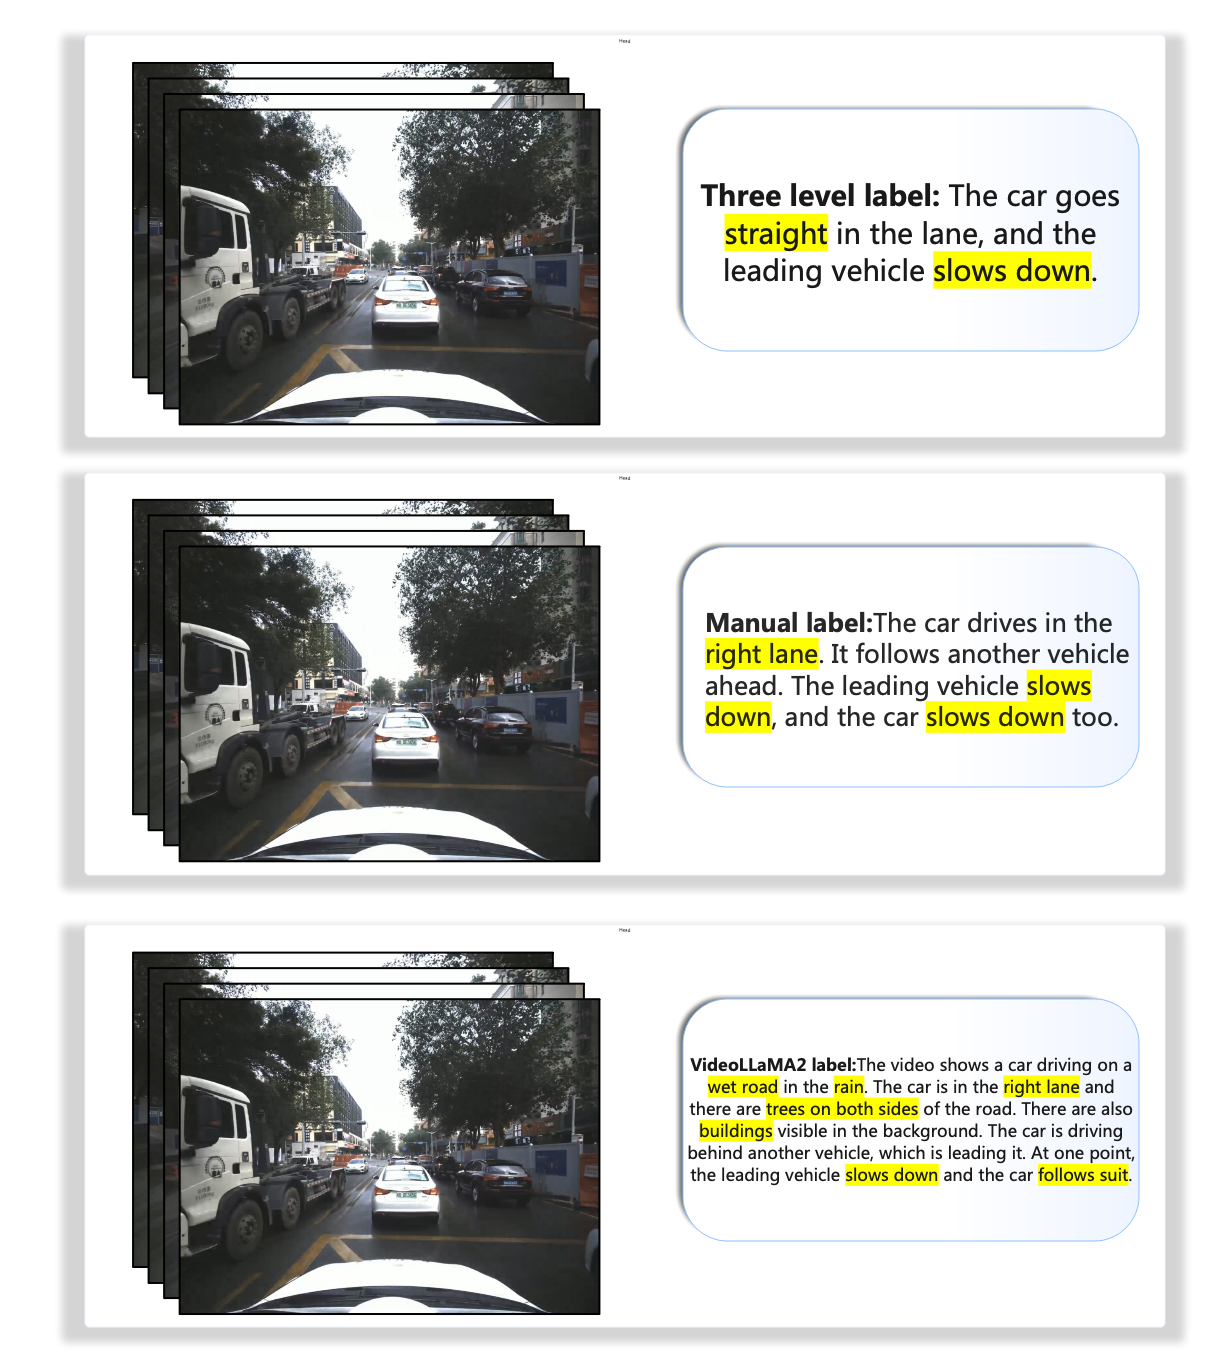
\includegraphics[width=0.9\linewidth]{images/Dataset.png}
    \caption{Examples of descriptions from the three annotation strategies: hierarchical labeling, manual annotation, and automatic generation using Video-LLaMA2.}
    \label{fig:2}
\end{figure}
\section{Experiments}
\subsection{Video-Text Retrieval Models Performance}
We evaluated two state-of-the-art video-text retrieval models (CLIP-ViP and VAST) on the Suscape dataset using different annotation methods. The performance was measured using standard retrieval metrics including Recall@1, Recall@5, Recall@10, Median Rank, and Mean Rank. The CLIP-ViP Model Performance is shown in \autoref{tab:clip_vip_performance} and the Vast Model Performance is shown in \autoref{tab:vast_performance}.


\begin{table*}[htbp]
\centering

\caption{Retrieval Performance Comparison Across Annotation Methods(Clip-Vip)}
\label{tab:clip_vip_performance}
\begin{tabular}{lccccc}
\toprule
\textbf{Annotation Method} & \textbf{Direction} & \textbf{Recall@1} & \textbf{Recall@5} & \textbf{Recall@10} & \textbf{Median Rank} \\
\midrule
Simple Labels & text-to-video & 5.65\% & 19.77\% & 33.33\% & 22.0 \\
Simple Labels & video-to-text & 1.63\% & 9.11\% & 19.21\% & 27.0 \\
DSL Labels & text-to-video & 5.65\% & 18.08\% & 30.51\% & 23.0 \\
DSL Labels & video-to-text & 1.63\% & 9.10\% & 19.19\% & 27.0 \\
Human Annotation & text-to-video & 14.12\% & 36.16\% & 49.15\% & 11.0 \\
Human Annotation & video-to-text & 4.65\% & 22.00\% & 40.97\% & 13.0 \\
Video-LLaMA2 Auto & text-to-video & 24.86\% & 57.06\% & 69.49\% & 4.0 \\
Video-LLaMA2 Auto & video-to-text & 26.08\% & 50.54\% & 69.02\% & 5.0 \\
\bottomrule
\end{tabular}

\end{table*}

\begin{table*}[htbp]
\centering
\caption{Retrieval Performance Comparison Across Annotation Methods(Vast)}
\label{tab:vast_performance}
\begin{tabular}{lccccc}
\toprule
\textbf{Annotation Method} & \textbf{Direction} & \textbf{Recall@1} & \textbf{Recall@5} & \textbf{Recall@10} & \textbf{Average} \\
\midrule
Human Annotation & text-to-video & 8.5\% & 35.0\% & 50.3\% & 31.3 \\
Human Annotation & text-to-video & 13.6\% & 42.4\% & 56.5\% & 37.5 \\
Video-LLaMA2 Auto & text-to-video & 23.7\% & 56.5\% & 73.4\% & 51.2 \\
Video-LLaMA2 Auto & text-to-video & 31.1\% & 65.0\% & 80.2\% & 58.8 \\
\bottomrule
\end{tabular}
\end{table*}


Key Findings are:
\begin{itemize}
    \item Both models showed significant improvement when using manual annotations compared to simple labels.
    \item Video-LLaMA2 automatic annotations achieved the best performance across all metrics.
    \item The VAST model generally outperformed CLIP-ViP in text-to-video retrieval tasks.
    \item The performance gap between text-to-video and video-to-text directions indicates there is still room for improvement in text encoder training.
\end{itemize}

\subsection{Evaluation of label accuracy under different questioning methods}
Next, we wanted to be able to use Video-LLaMA2 again to generate tertiary labels on top of the known secondary labels, using a questioning method that mimicked DriveLM's Chain of Mind model. 

\begin{itemize}
    \item Implementation:
        \begin{itemize}
            \item Progressive label refinement via interactive QA cycles
            \item Secondary-label-guided tertiary label generation
            \item Multi-strategy questioning for optimization
        \end{itemize}
    \item Validation:
        \begin{itemize}
            \item Video-LLaMA2 proves label-assisted generation viability
            \item DriveLM evidences Chain-of-Thought efficacy
        \end{itemize}
\end{itemize}

\subsubsection{Type 1: Basic questions}

\begin{itemize}
    \item Standardized question set: Employs a fixed yet concise list covering basic vehicle interaction contexts, though without refined label definitions
    \item Core scenario focus: Questions center on critical elements including: Leading vehicle position, Traffic signals, Obstacles, Lane incursion/exit events, Pedestrian crossings, Vehicle status
    \item Structured decision-making: Concludes with multiple-choice questions to determine tertiary labels
\end{itemize}

See full question list of Type 1 in \ref{appendix:qa_list1})

\begin{figure}
    \centering
    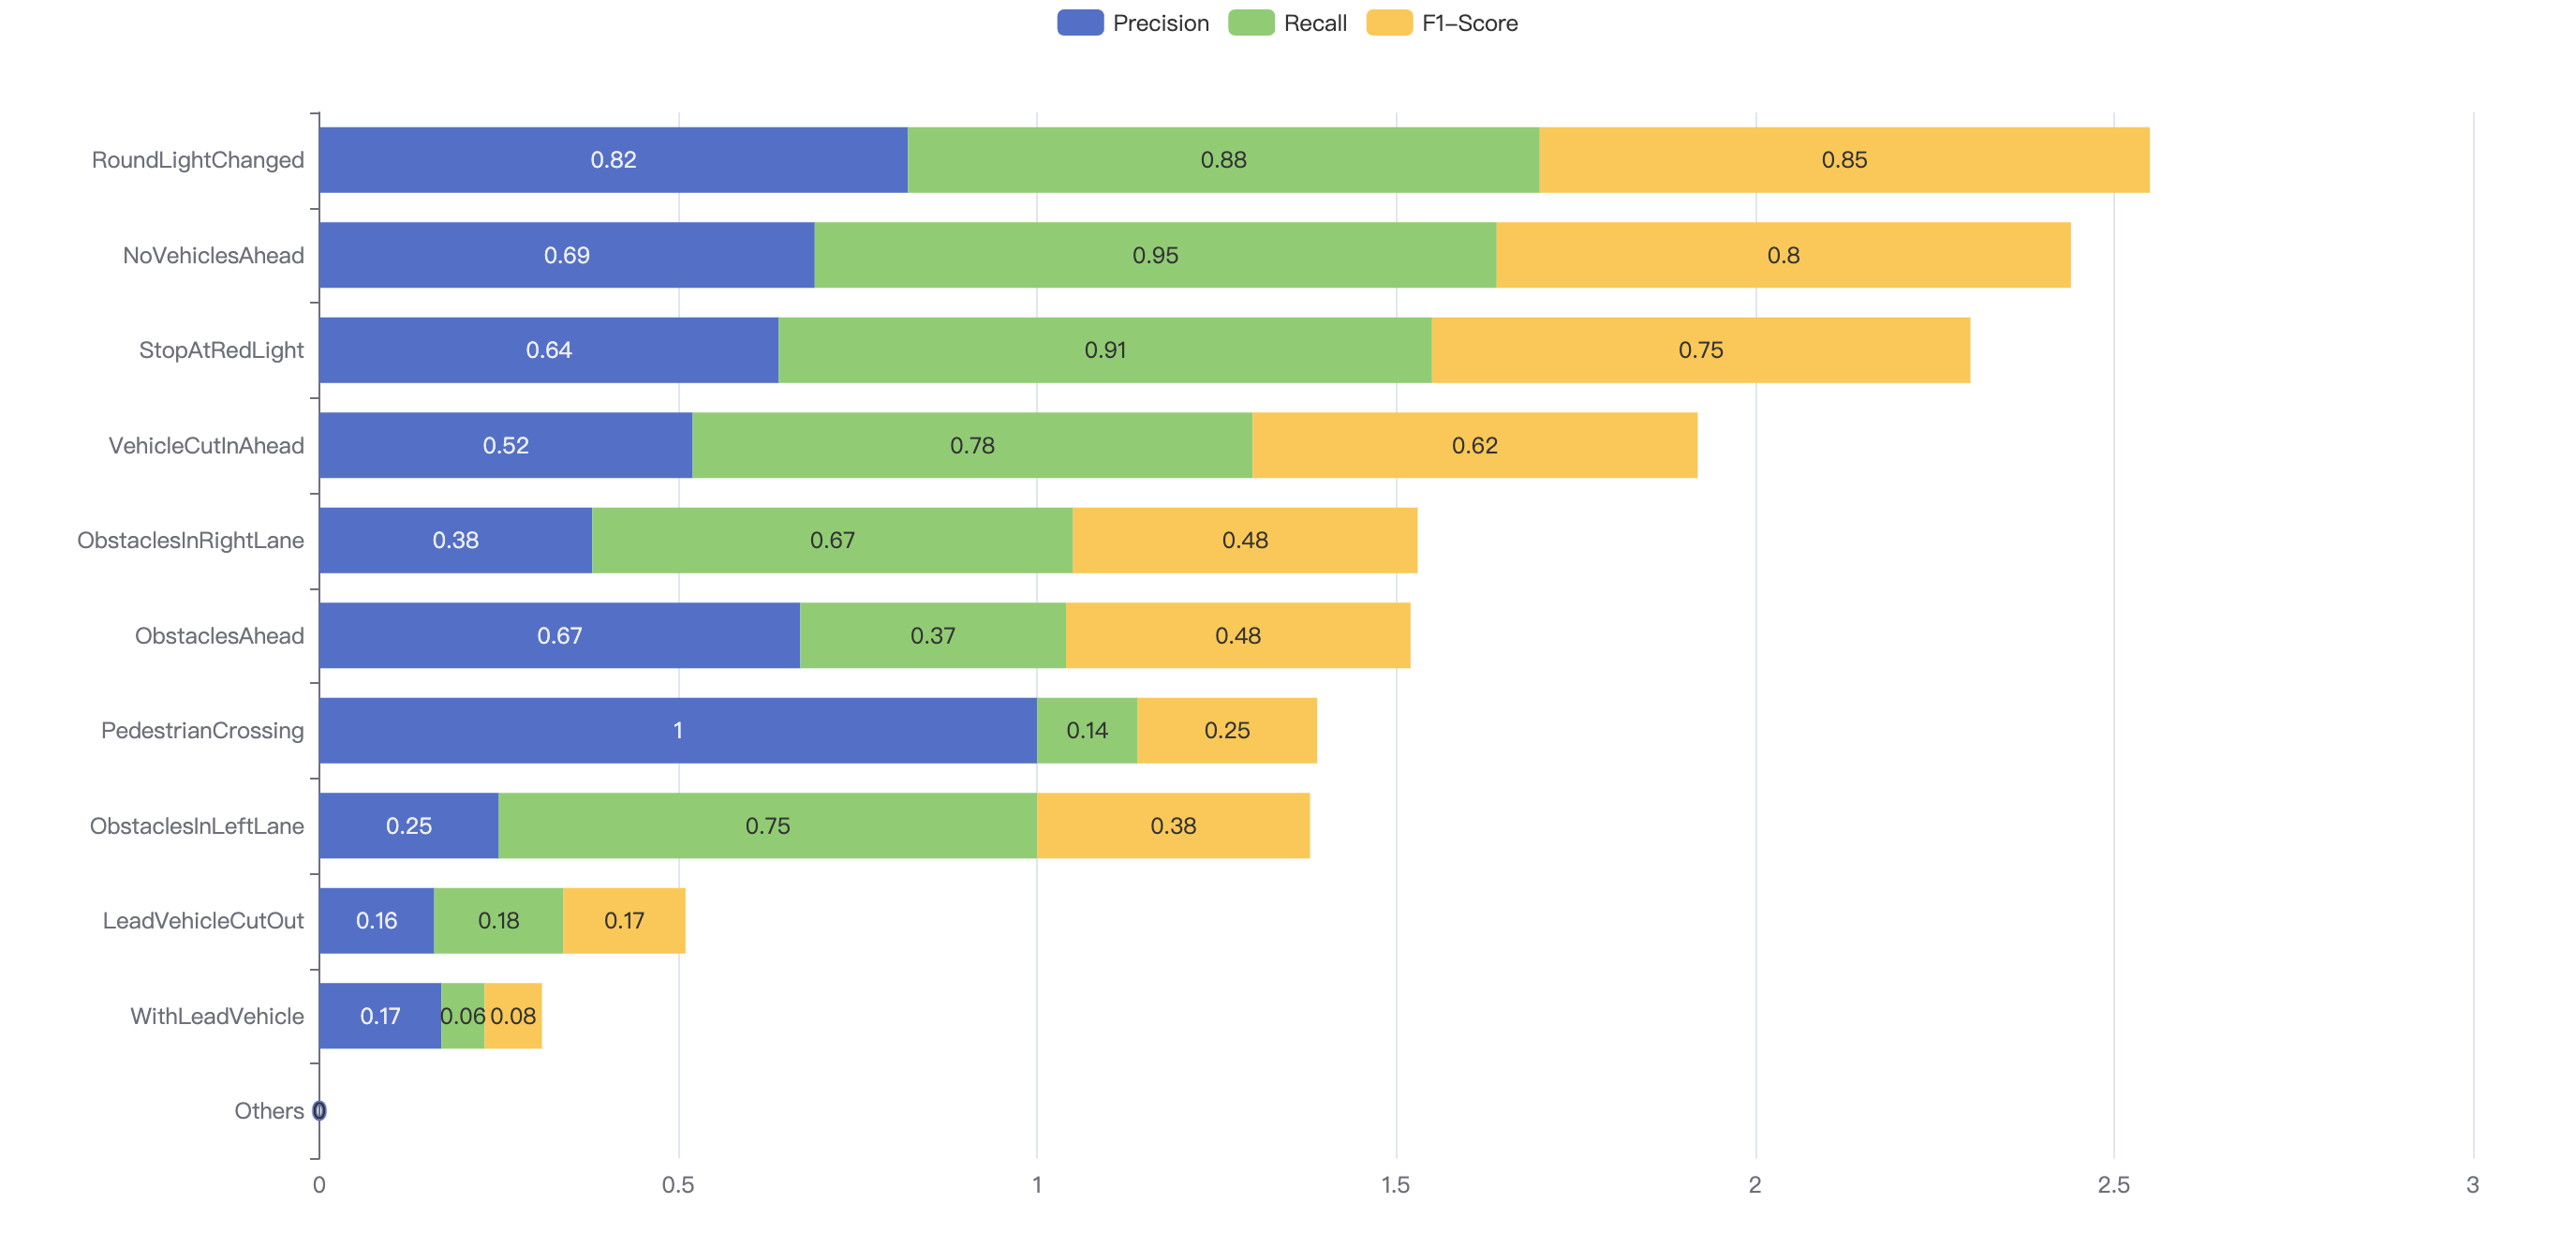
\includegraphics[width=0.9\linewidth]{images/result1.png}
    \caption{Accuracy of three-level label prediction using Type 1}
    \label{fig:3}
\end{figure}

\subsubsection{Type 2: Enhanced questions with definitions}
\begin{itemize}
    \item Enhanced label definitions: Explicit explanations of tertiary-level tags are incorporated to enable more comprehensive model understanding

    \item Chain-of-Thought prompting: Multi-step questioning progressively guides the model through refined judgment processes

    \item Multi-dimensional coverage: Encompasses critical driving aspects including: Lane incursion/exit maneuvers, Vehicle stopping scenarios, Wrong-way driving detection, Traffic signal interpretation, Obstacle recognition, Pedestrian interactions, Trajectory analysis
\end{itemize}

See full question list of Type 2 in \ref{appendix:qa_list2})

\begin{figure}
    \centering
    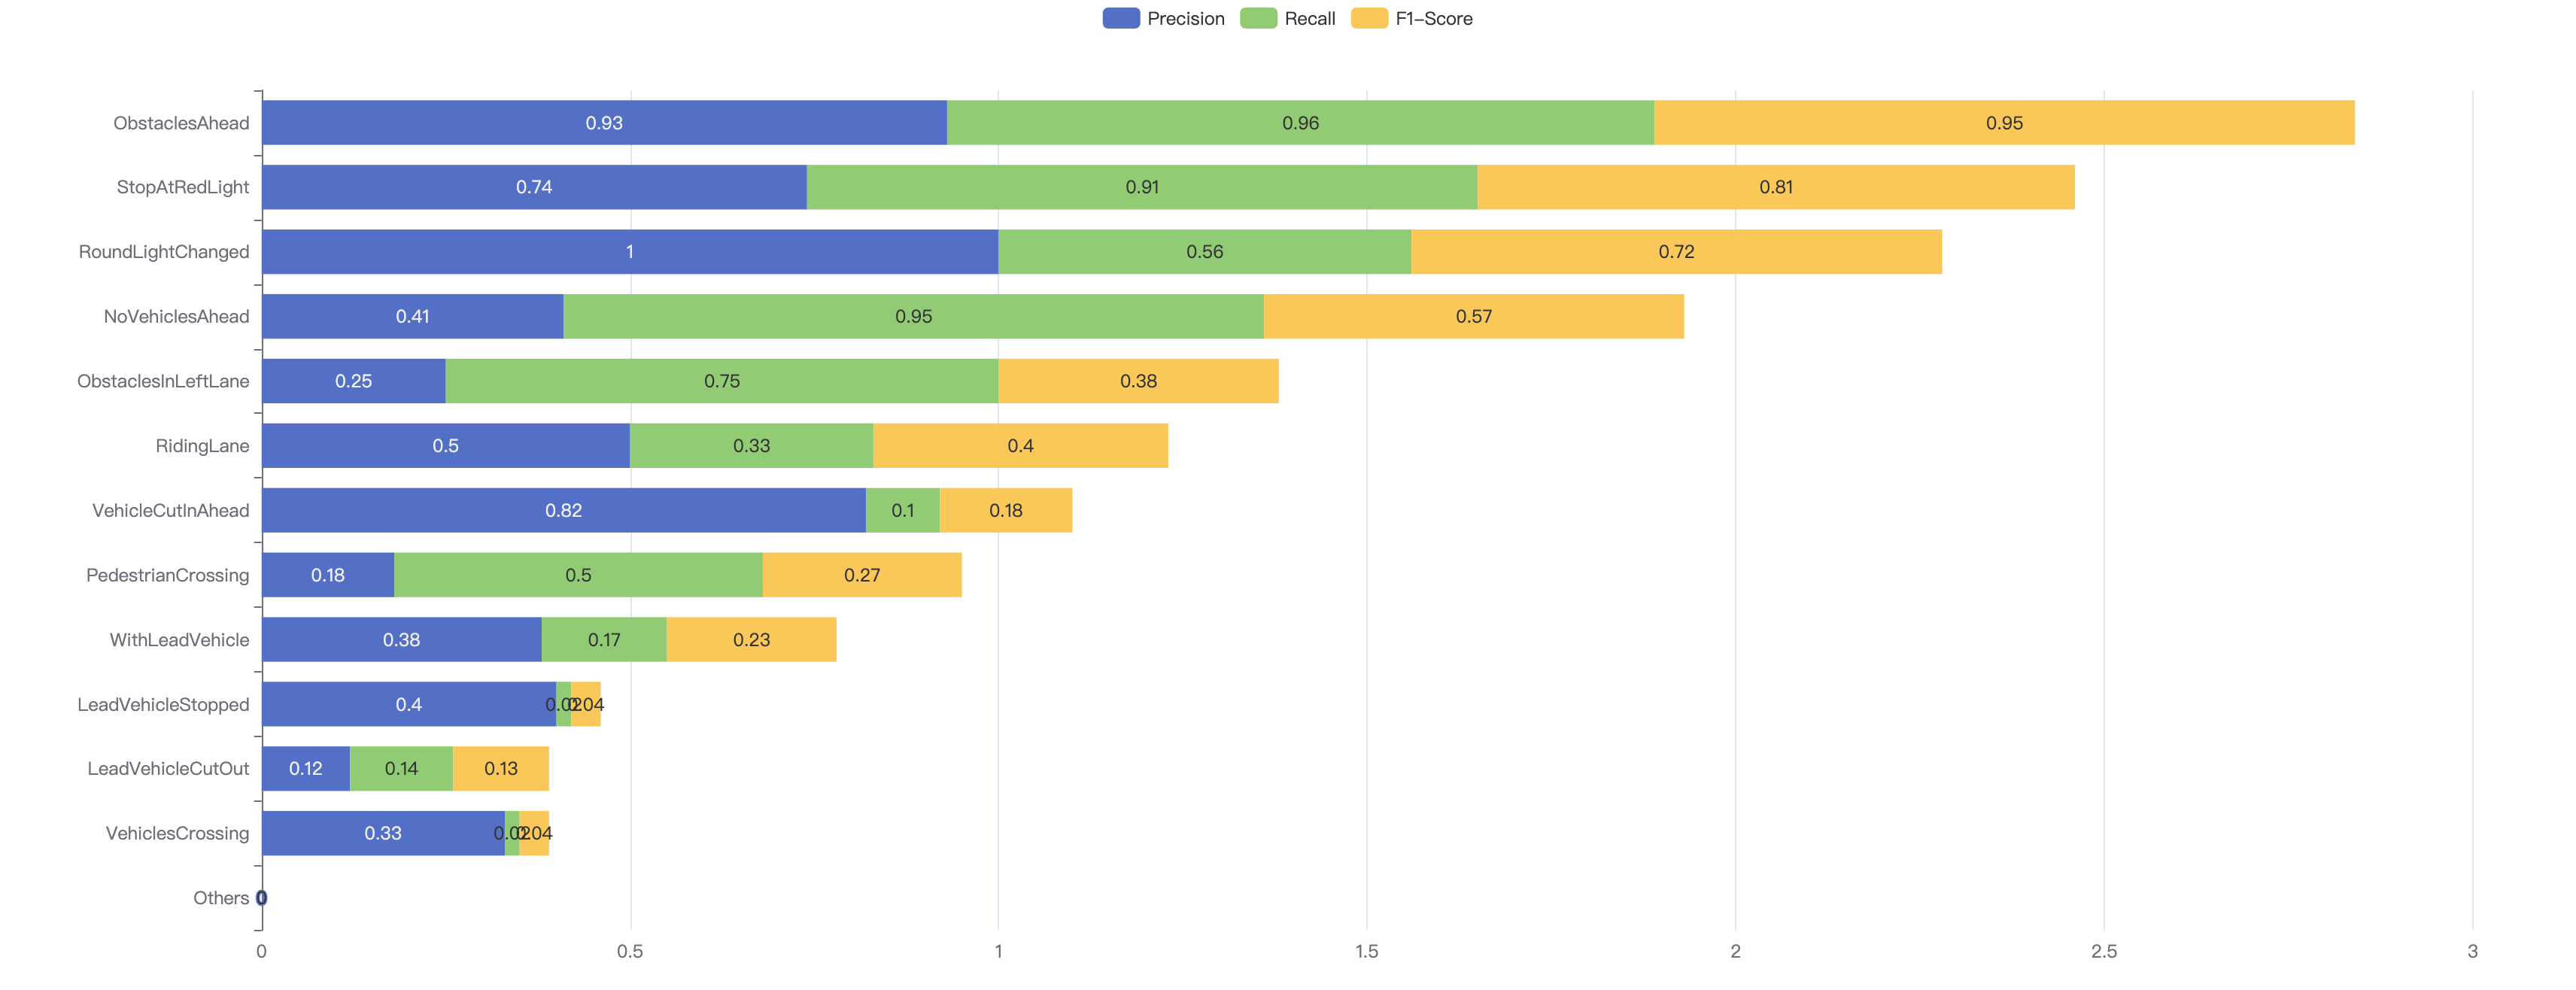
\includegraphics[width=0.9\linewidth]{images/result2.png}
    \caption{Accuracy of three-level label prediction using Type 2}
    \label{fig:4}
\end{figure}

\subsubsection{Type 3: Contextualized Branch Questions}
\begin{itemize}
    \item Hierarchical question design: Customized question sets tailored to different secondary-level labels for precise scenario targeting
    \item Dynamic branching protocol: Adaptive multi-round questioning paths that evolve based on contextual responses
    \item Semantic augmentation: Leverages secondary label semantics to optimize tertiary-level label determination accuracy
    
\end{itemize}

See full question list of Type 3 in \ref{appendix:qa_list3})

\begin{figure}
    \centering
    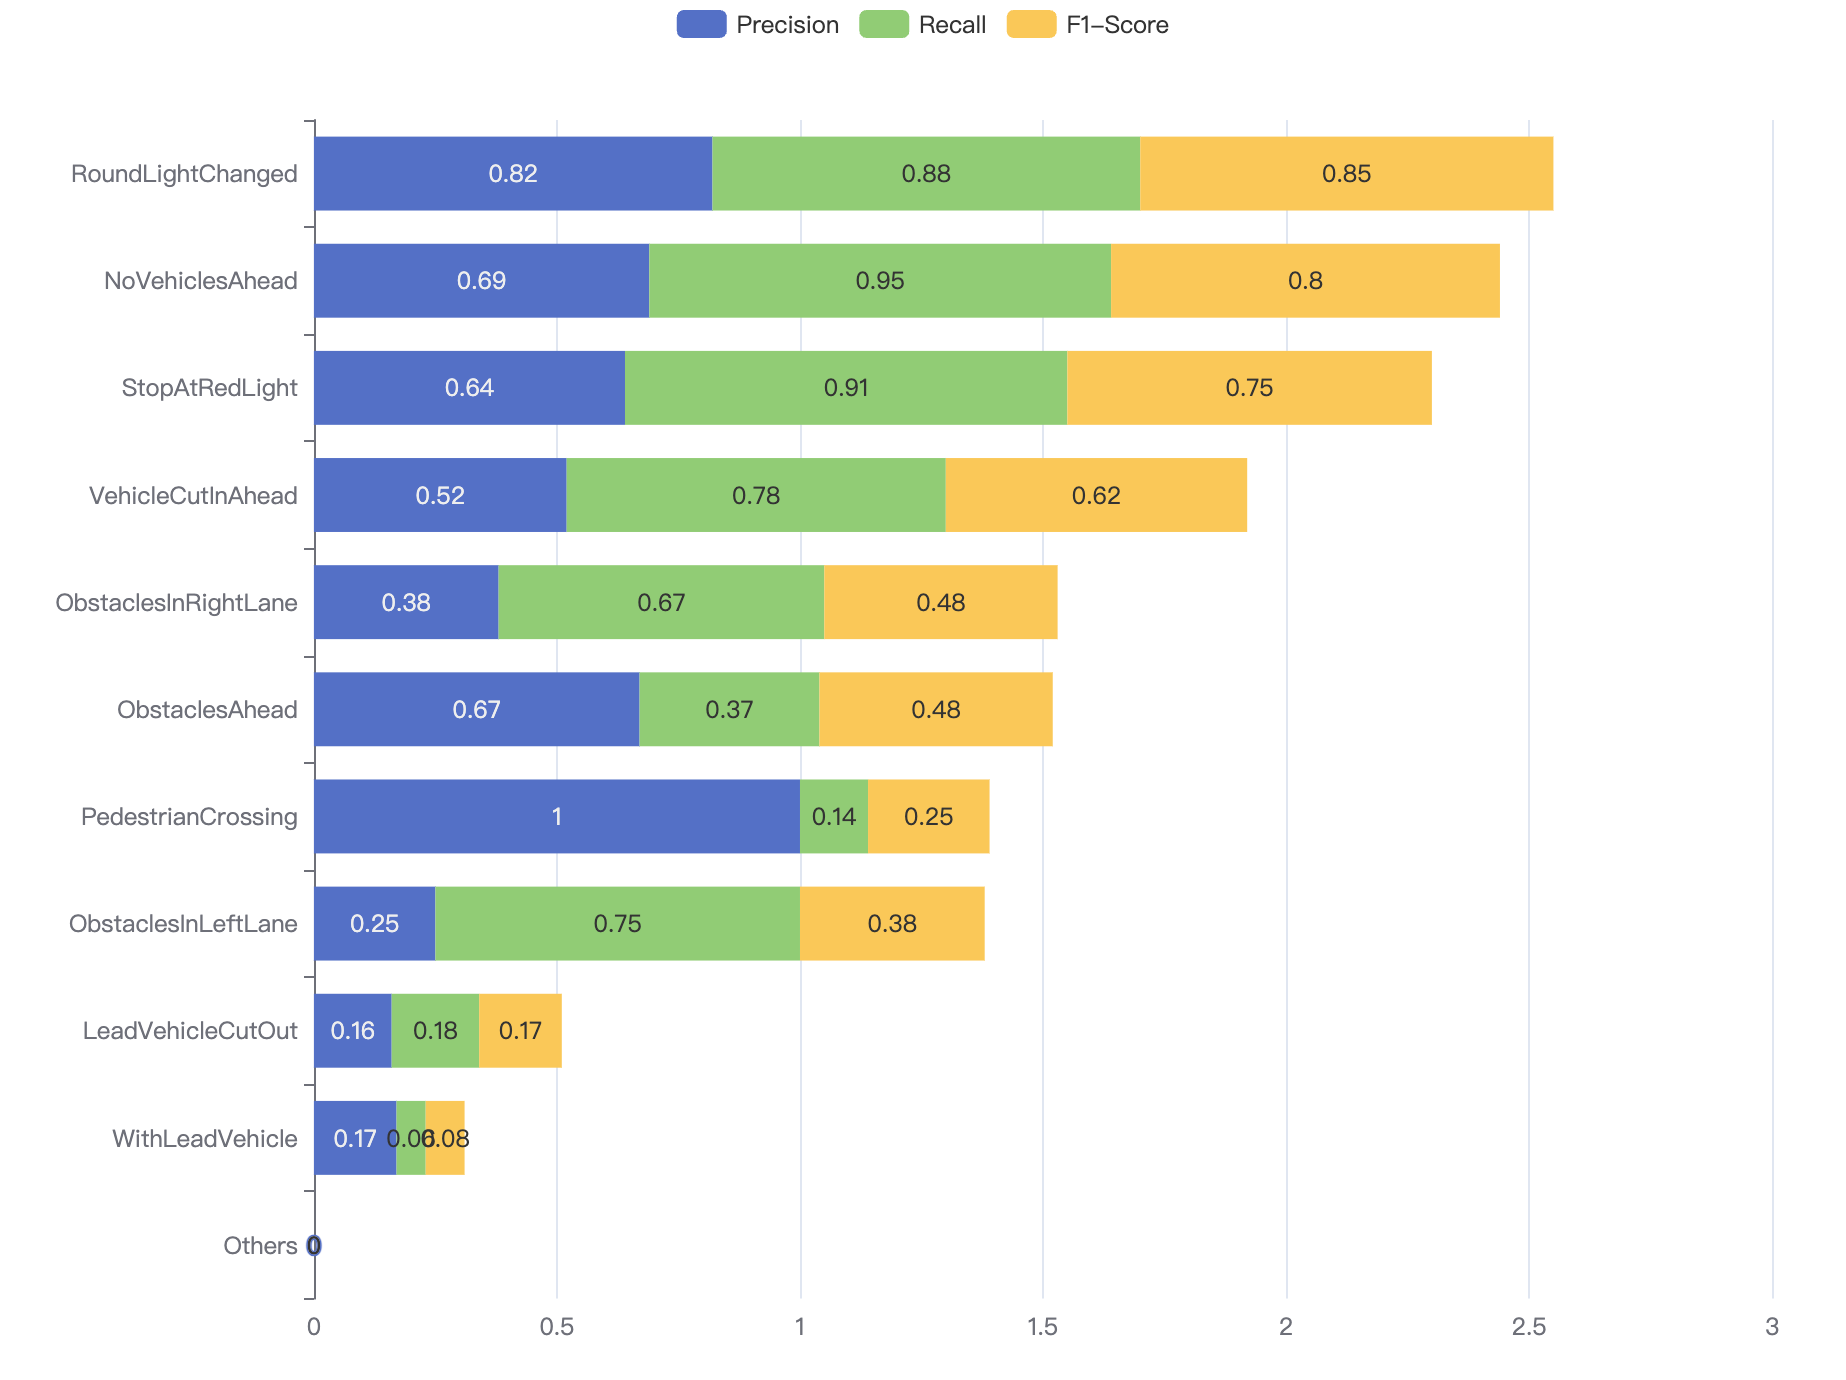
\includegraphics[width=0.9\linewidth]{images/result3.png}
    \caption{Accuracy of three-level label prediction using Type 3}
    \label{fig:5}
\end{figure}


\subsection{Fine-tuning for Video-LLaMA2 and InterVL2.5}
In order to further improve the accuracy of tertiary label generation, we have fine-tuned Video-LLaMA2 and InternVL2.5. Imitate the chain of thought structure of DriveLM, and organize fine - tuning data into a hierarchical, multi - turn interactive Q\&A form, which facilitates the model to gradually reason about the key semantic information in the video. Each dialogue contains multiple rounds of Q\&A, capturing information at stages such as Perception, Prediction, Planning, Behavior, and Motion layer by layer.Distinguish types of questions to assist the model in understanding temporal and logical dependencies.Enhance the model's ability to understand and reason about details and complex scenarios.

\begin{figure}
    \centering
    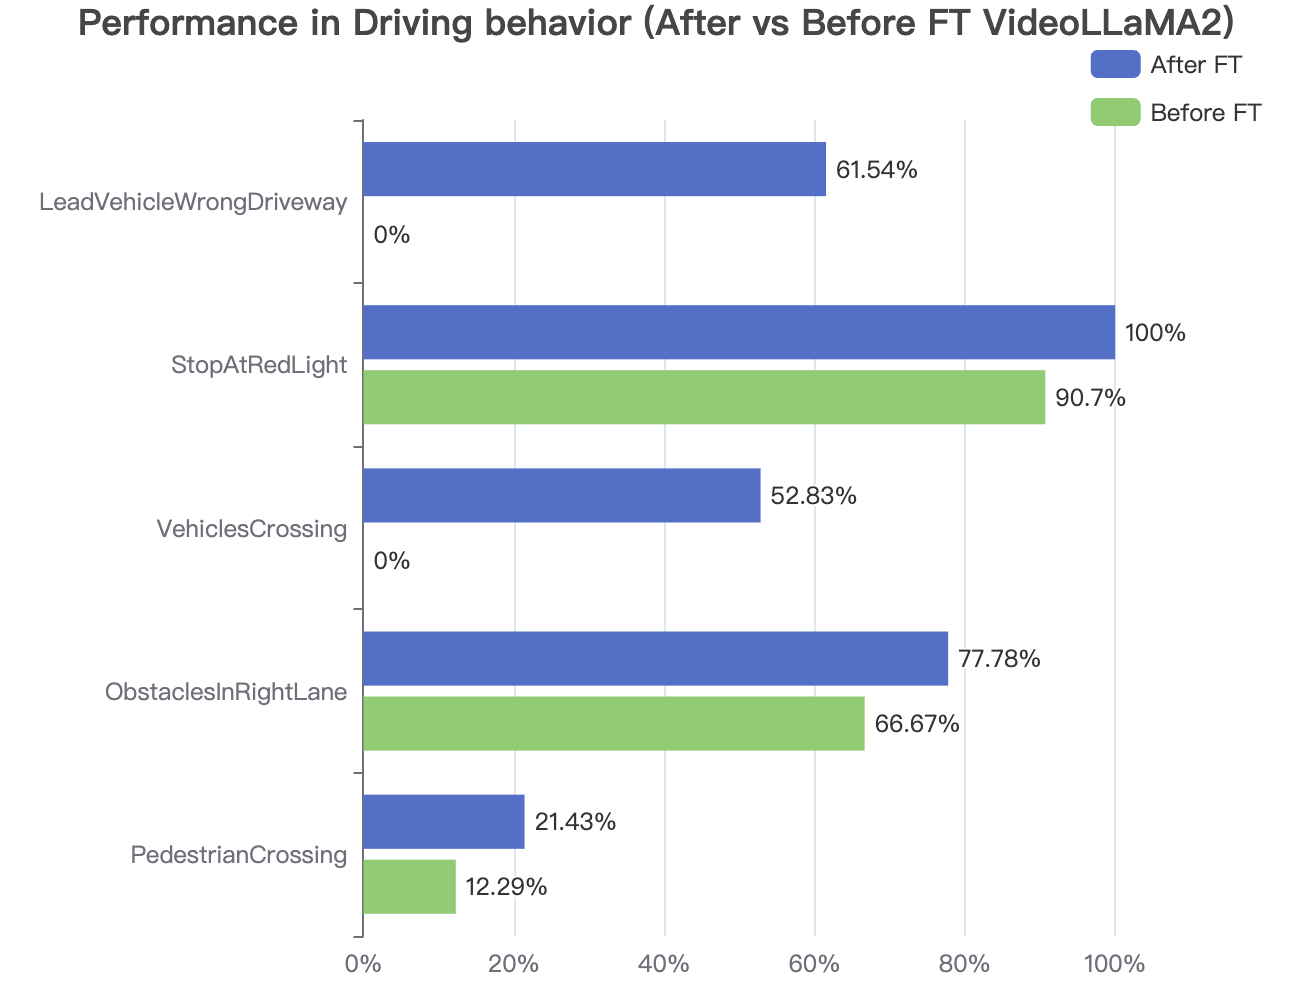
\includegraphics[width=0.5\linewidth]{images/Performance in Driving behavior(VideoLLaMA2).png}
    \caption{Performance after finetuing(Video-LLaMA2)}
    \label{fig:6}
\end{figure}

\begin{figure}
    \centering
    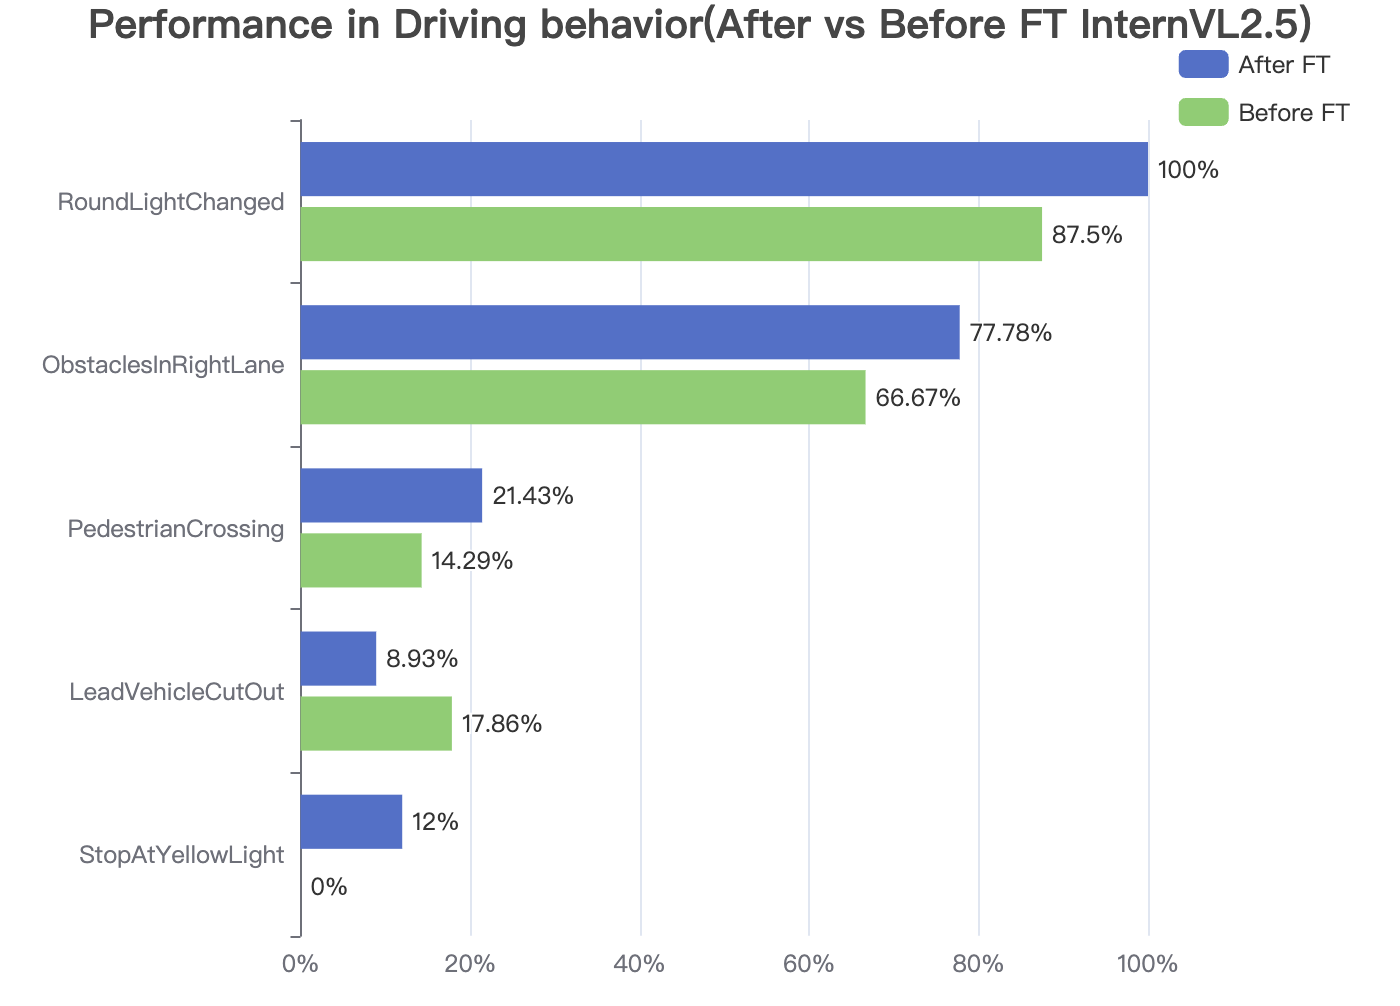
\includegraphics[width=0.5\linewidth]{images/Performance in Driving behavior(InternVL2.5).png}
    \caption{Performance after finetuing(InterVL2.5)}
    \label{fig:7}
\end{figure}

\section{Conclusion}

Autonomous driving video retrieval presents unique challenges due to the complexity of real-world driving scenarios and the scarcity of high-quality annotated datasets. In this work, we explored the potential of multimodal large language models (MLLMs) to bridge the gap between visual perception and textual understanding in autonomous driving contexts. By leveraging a carefully curated dataset with optimized annotations, combining human expertise and automated refinement using Video-LLama2, we demonstrated that pretrained MLLMs can be effectively adapted for domain-specific video retrieval tasks.

Our experiments with two state-of-the-art MLLMs (Vast and Clip-Vip) revealed that fine-tuning on high-quality annotated data significantly improves retrieval accuracy, validating the importance of robust dataset construction. Additionally, our work establishes a benchmark for future research in autonomous driving video understanding, providing a foundation for developing more interpretable and scalable retrieval systems.

Moving forward, we anticipate that further advancements in MLLMs, combined with more sophisticated annotation pipelines, will enhance the generalization capabilities of autonomous driving systems. Future research could explore dynamic annotation strategies, real-time retrieval optimization, and the integration of multi-sensor data (e.g., LiDAR and radar) to further improve model performance in complex driving environments.

Ultimately, this study highlights the critical role of high-quality data and domain-specific adaptation in advancing autonomous driving technologies, paving the way for safer and more intelligent transportation systems.



\appendices
\section{Complete Three-Level Label Structure}
\label{appendix:three_level_labels}

\begin{enumerate}
    \item GoStraight
    \begin{enumerate}
        \item InLane
        \begin{enumerate}
            \item LeadVehicleConstant
            \item LeadVehicleCutOut
            \item VehicleCutInAhead
            \item LeadVehicleDecelerating
            \item LeadVehicleStopped
            \item LeadVehicleAccelerating
            \item LeadVehicleWrongDriveway
            \item PedestrianCrossing
        \end{enumerate}
        \item ChangingLaneLeft
        \begin{enumerate}
            \item ObstaclesAhead
            \item RidingLane
            \item ObstaclesInLeftLane
        \end{enumerate}
        \item ChangingLaneRight
        \begin{enumerate}
            \item ObstaclesAhead
            \item ObstaclesInRightLane
        \end{enumerate}
        \item ChangingTurnLeft
        \item ChangingTurnRight
        \item ChangingStop
        \item Avoidance
        \item RidingLane
    \end{enumerate}
    
    \item Crossing
    \begin{enumerate}
        \item StopAndWait
        \begin{enumerate}
            \item StopAtRedLight
            \item StopAtYellowLight
            \item StopAtFlashGreenLight
            \item LeadVehicleStopped
            \item PedestrianCrossing
            \item VehiclesCrossing
        \end{enumerate}
        \item Starting
        \begin{enumerate}
            \item ArrowLightChanged
            \item RoundLightChanged
        \end{enumerate}
        \item EnterWaitingArea
        \begin{enumerate}
            \item RoundLightChanged
        \end{enumerate}
        \item GoStraight
        \begin{enumerate}
            \item NoVehiclesAhead
            \item WithLeadVehicle
            \item VehiclesCrossing
        \end{enumerate}
        \item TurnLeft
        \begin{enumerate}
            \item NoVehiclesAhead
            \item WithLeadVehicle
            \item VehiclesCrossing
        \end{enumerate}
        \item TurnRight
        \begin{enumerate}
            \item NoVehiclesAhead
            \item WithLeadVehicle
            \item VehiclesCrossing
        \end{enumerate}
        \item UTurn
        \begin{enumerate}
            \item NoVehiclesAhead
            \item WithLeadVehicle
            \item VehiclesCrossing
        \end{enumerate}
    \end{enumerate}
    
    \item Bridge
    \begin{enumerate}
        \item DriveIn
        \item DriveOut
    \end{enumerate}
    
    \item SlipRoad
    \begin{enumerate}
        \item DriveIn
        \item DriveOut
        \item Driving
    \end{enumerate}
\end{enumerate}


\section{Complete Question List 1}
\label{appendix:qa_list1}

\begin{enumerate}
    \item Is there a leading vehicle ahead driving in the same lane as the ego vehicle?
    \item Is there a traffic light ahead?
    \item Are there obstacles ahead?
    \item What is the shape of the traffic light? (Round/Arrow)
    \item Are there vehicles cutting into or out of the lane ahead?
    \item Does the leading vehicle stop?
    \item Are there vehicles crossing the road ahead?
    \item Is there a pedestrian crossing the road?
    \item Final label selection
\end{enumerate}


\section{Complete Question List 2}
\label{appendix:qa_list2}

\begin{enumerate}

    \item Is there a leading vehicle in the current lane ahead? A leading vehicle means a vehicle or a motorcycle driving in the front exactly in the same lane as the ego vehicle or a vehicle driving in front of and in the same direction as the ego vehicle when crossing.
    \item Is there a leading vehicle or a leading motorcycle cutting into the lane of the ego vehicle? Cutting in means the leading vehicle enters the lane of the ego vehicle from the adjacent lane ahead.
    \item Is there a leading vehicle or a leading motorcycle cutting out of the lane of the ego vehicle? Cutting out means the leading vehicle leaves from the lane of the ego vehicle to the adjacent lane ahead.
    \item Does the leading vehicle stop?
    \item Is there a traffic light ahead? What is the shape, round or arrow?
    \item Does the ego vehicle stop? If so, why does the ego vehicle stop?
    \item Is there a vehicle or a motorcycle in the same lane as the ego vehicle but driving in the opposite direction or stopping in the lane and heading to a different direction that will influence the ego vehicle? Is there a crossing with vehicles and motorcycles driving in different directions with the ego vehicle?
    \item Are there obstacles on the current road? Obstacles means objects excluding vehicles, motorcycles and pedestrians. If so, is the obstacle on the current lane, the left lane or the right lane?
    \item Are there pedestrians crossing ahead that will influence the ego vehicle? Pedestrians here means person.
    
    \item Is the ego vehicle riding the lane? Riding the lane means the ego vehicle is driving in the middle of two lanes.
    \item According to the previous questions and the corresponding answers, and the content of the video, which label fits the video best, LeadVehicleCutOut, VehicleCutInAhead, LeadVehicleStopped, LeadVehicleWrongDriveway or PedestrianCrossing?
\end{enumerate}


\section{Complete Question List 3}
\label{appendix:qa_list3}
\begin{enumerate}
    \item InLane:
    \begin{enumerate}
        \item Is there any vehicle in front of the ego vehicle?
        \item If there are pedestrians crossing in front of the ego vehicle, answer ”pedestrian crossing”. Otherwise skip.
        \item What does the vehicle in front do? Change lanes, stop, or drive in the opposite direction?
        \item If the vehicle in front changes lanes, does it enter the current lane (cutting in) or leave it (cutting out)?
        \item Does the vehicle in front stop?
        \item Does the vehicle in front drive in the opposite direction?
    \end{enumerate}
    \item ChangingLaneLeft:
        \begin{enumerate}
            \item Are there obstacles ahead? Obstacles exclude vehicles and pedestrians (e.g., bicycles).
            \item If yes, are the obstacles in the left lane or directly ahead?
            \item If no obstacles, is the ego vehicle riding the lane?
        \end{enumerate}
    \item StopAndWait:
    \begin{enumerate}
        \item Is there a traffic light ahead?
        \item What is the color of the traffic light? Red, Yellow or Green?
        \item If no red light, are there pedestrians crossing?
        \item If no pedestrians, are there vehicles crossing ahead? 
    \end{enumerate}

    \item Starting:
    \begin{enumerate}
        \item What color is the traffic light?
        \item Is the traffic light changing? If not, skip.
        \item What is the shape of the traffic light? Round or Arrow?
    \end{enumerate}

    \item EnterWaitingArea:
    \begin{enumerate}
        \item What is the shape of the traffic light? Round or Arrow?
    \end{enumerate}

    \item GoStraight / TurnLeft / TurnRight / UTurn:
    \begin{enumerate}
        \item Are there vehicles ahead or not during the maneuver?
        \item If yes, are the vehicles leading the ego vehicle or crossing in different directions?
    \end{enumerate}
  
    \end{enumerate}

\balance
\bibliographystyle{IEEEtran}
\bibliography{reference}

\end{document}